As PECs become increasingly complex, intelligent maintenance has emerged as a key element for ensuring long-term reliability, safety, and cost efficiency. 
While the control layer governs real-time dynamics, the maintenance layer focuses on monitoring equipment health, anticipating failures, and optimizing life-cycle performance. 
DRL enables adaptive and data-driven maintenance strategies that extend beyond static, rule-based, or threshold-driven paradigms. 
Fig.~\ref{fig:maintenance} presents the workflow of DRL-based maintenance in PECs, integrating data acquisition, feature extraction, decision-making, and maintenance action planning.

% \begin{figure*}[t]
%   \centering
%   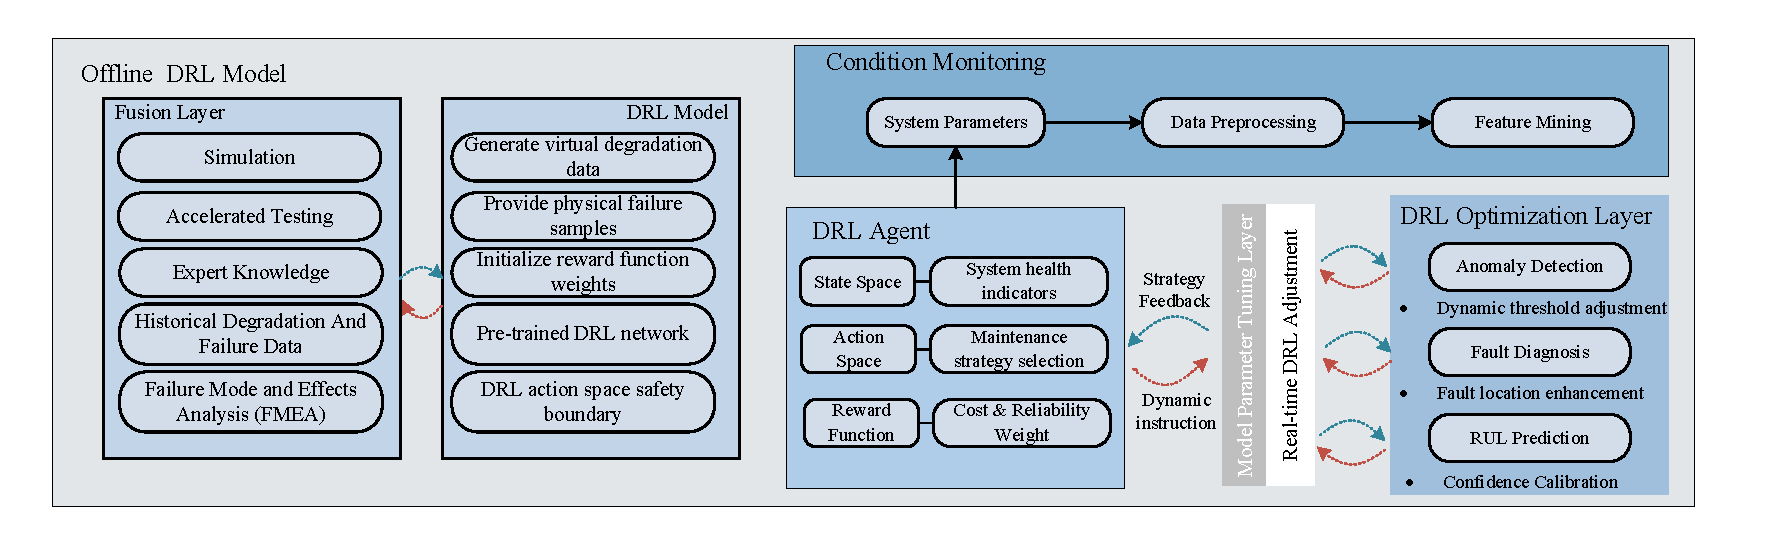
\includegraphics[width=\textwidth]{fig/maintenance.pdf}
%   \caption{Workflow of DRL-enabled maintenance for PECs.}
%   \label{fig:maintenance}
% \end{figure*}

% \noindent

% In PECs maintenance, DRL can operate at two distinct levels of abstraction: 
% (1) as a \textit{policy-level agent} that learns optimal maintenance actions, and 
% (2) as a \textit{representation-level learner} that enhances feature extraction or anomaly perception. 
% Clarifying this distinction is essential for evaluating each study’s methodological focus and its role in the maintenance hierarchy.

% \begin{table}[t]
% \centering
% \caption{Comparison Between Policy-Level and Representation-Level DRL in PEC Maintenance}
% \label{tab:drl_roles_maintenance}
% \renewcommand{\arraystretch}{1.2}
% \resizebox{\linewidth}{!}{
% \begin{tabular}{@{}p{2.8cm}p{5.8cm}@{}}
% \toprule
% \textbf{Category} & \textbf{Key Characteristics in Maintenance Applications} \\ 
% \midrule
% \textbf{Policy-Level DRL} & Learns maintenance or resource-allocation policies based on state–reward feedback; directly selects inspection, replacement, or repair actions. 
% Examples include PPO–LSTM for dynamic maintenance scheduling~\cite{ong2021deep} and TD3 for opportunistic maintenance planning~\cite{najafi2023deep}. \\ 
% \textbf{Representation-Level DRL} & Embeds reinforcement mechanisms within deep networks to learn discriminative health-state features; enhances perception for monitoring or diagnosis. 
% Examples include DANN-based transfer DRL for cross-domain fault recognition~\cite{saleem2024transrul} and attention-guided DRL for degradation feature extraction~\cite{xu2024comparative}. \\ 
% \bottomrule
% \end{tabular}}
% \end{table}

% The applications of DRL in converter maintenance can be grouped into three interrelated domains:
% \begin{enumerate}
%   \item \textbf{Condition Monitoring}: continuous assessment of converter health through sensor data and latent feature representation;
%   \item \textbf{Anomaly Detection and Fault Diagnosis}: identification and localization of deviations from nominal operation;
%   \item \textbf{Remaining Useful Life (RUL) Prediction}: estimation of degradation trajectories to support predictive and prescriptive maintenance.
% \end{enumerate}
% These domains collectively form a hierarchical pipeline that connects observation, interpretation, and prediction across the converter life cycle.

% %%%%%%%%%%%%%%%%%%%%%%%%%%%%%%%%%%%%%%%%%%%%%%%%%%%
% \subsection{Condition Monitoring}
% \label{Condition_Monitoring}
% %%%%%%%%%%%%%%%%%%%%%%%%%%%%%%%%%%%%%%%%%%%%%%%%%%%

% Condition monitoring provides the foundation for intelligent maintenance by enabling continuous evaluation of system health under dynamic operating conditions. 
% Traditional thresholding or statistical methods often fail to generalize across nonlinear or time-varying environments. 
% Recent works have coupled DRL with deep representation learning to enhance adaptability and scalability in converter monitoring~\cite{xu2024comparative}. 
% In multi-source energy systems such as hybrid microgrids, DRL-based agents extract high-level features directly from raw data streams and transfer monitoring policies across distinct operating regimes.

% To improve generalization under limited data, transfer learning and domain adaptation have been integrated with DRL frameworks. 
% Techniques such as fine-tuning and domain-adversarial neural networks (DANN) enhance cross-system fault recognition~\cite{saleem2024transrul}. 
% In HVAC benchmarks, DANN-based DRL achieved over 93~\% average fault detection accuracy with minimal labeled data, illustrating its transferability to converter diagnostics and robustness against distributional shifts.

% Transformer architectures have also been applied to extract temporal dependencies and long-range correlations within operational sequences. 
% Through self-attention mechanisms, DRL-enhanced transformers selectively emphasize critical time intervals, improving sensitivity to early-stage degradation. 
% These advances collectively enable accurate, adaptive, and generalizable health-state estimation, forming the basis for subsequent anomaly detection and predictive maintenance.

% %%%%%%%%%%%%%%%%%%%%%%%%%%%%%%%%%%%%%%%%%%%%%%%%%%%
% \subsection{Anomaly Detection and Fault Diagnosis}
% \label{sec:fault_diagnosis}
% %%%%%%%%%%%%%%%%%%%%%%%%%%%%%%%%%%%%%%%%%%%%%%%%%%%

% Following health-state awareness, the next stage focuses on anomaly detection and fault diagnosis. 
% Conventional model-based or rule-driven methods often exhibit limited robustness in nonlinear converter environments. 
% DRL addresses this limitation by learning diagnostic policies directly from high-dimensional sensor data while optimizing corrective decisions.

% A representative hybrid CNN–RNN DRL framework~\cite{nevisi2025evolutionary} combines convolutional layers for spatial feature extraction and recurrent units for temporal reasoning, with an evolutionary bee-colony optimizer for hyperparameter tuning. 
% Evaluated on multiple smart-grid datasets, this method achieved over 96~\% classification accuracy and maintained low false-alarm rates, outperforming GAN- and transformer-based baselines.  

% For multi-unit systems with economic interdependence, a semi-Markov DRL framework integrates proportional hazards modeling to capture condition-dependent degradation~\cite{najafi2023deep}. 
% The learned policy derives opportunistic maintenance strategies that minimize long-term cost while accounting for component aging correlations. 
% In higher-level applications, PPO–LSTM agents have been used for dynamic maintenance resource allocation~\cite{ong2021deep}, improving efficiency by 53–65~\% relative to conventional scheduling approaches.  

% Specialized diagnostic tasks also benefit from DRL’s adaptive exploration. 
% In electromagnetic susceptibility testing, TD3-based agents autonomously design excitation waveforms that expose converter vulnerabilities, achieving faster convergence and higher detection sensitivity~\cite{chen2024determining}. 
% Similarly, reinforcement learning has been applied to excitation design for system identification in Li-ion battery systems~\cite{huang2023reinforcement}, a methodology readily extendable to converter magnetic and capacitive components.  

% These developments demonstrate that DRL unifies perception, fault detection, and maintenance decision-making within a coherent, data-driven framework. 
% Remaining challenges include policy interpretability, limited fault-data availability, and achieving real-time execution under embedded hardware constraints.

% %%%%%%%%%%%%%%%%%%%%%%%%%%%%%%%%%%%%%%%%%%%%%%%%%%%
% \subsection{Remaining Useful Life Prediction}
% \label{sec:rul_prediction}
% %%%%%%%%%%%%%%%%%%%%%%%%%%%%%%%%%%%%%%%%%%%%%%%%%%%

% Once fault conditions are identified, the subsequent stage involves predicting the RUL of key components to support predictive maintenance. 
% Accurate RUL estimation ensures optimal component utilization, reduces unplanned downtime, and enhances safety. 
% Traditional physics-based models often require extensive parameterization and exhibit poor adaptability under variable stress conditions, whereas DRL and transformer-based approaches offer flexible, data-driven alternatives.

% An actor–critic DDPG framework~\cite{haque2021deep} was developed for degradation-aware control of solid-state transformers (SSTs), dynamically adjusting phase-shift angles according to real-time health indicators. 
% Experimental validation on a 5~kW GaN-based SST prototype demonstrated a 3~\% improvement in efficiency and reduced thermal stress without explicit degradation modeling, illustrating the potential for RUL-integrated control.  

% Complementarily, transformer-based sequence models such as the Trans-RUL framework~\cite{saleem2024transrul} estimate component lifetime using dual encoders and multi-head attention. 
% Evaluated on the CALCE CS$_2$ dataset, this model reduced mean absolute error and root mean square error compared with convolutional baselines while maintaining a lightweight structure suitable for embedded deployment.  

% These two directions—control-integrated lifetime extension and sequence-based degradation modeling—jointly advance RUL prediction toward fully autonomous, self-adaptive maintenance in PECs.

% %%%%%%%%%%%%%%%%%%%%%%%%%%%%%%%%%%%%%%%%%%%%%%%%%%%
% \subsection{Discussion and Future Outlook}
% \label{sec:maintenance_discussion}
% %%%%%%%%%%%%%%%%%%%%%%%%%%%%%%%%%%%%%%%%%%%%%%%%%%%

% DRL-enabled maintenance represents a paradigm shift in the reliability engineering of PECs. 
% Across condition monitoring, anomaly diagnosis, and RUL prediction, DRL provides a unified framework that connects perception, reasoning, and decision-making throughout the converter life cycle.  
% Condition monitoring benefits from attention-based feature learning and domain transferability; anomaly detection leverages sequential policy optimization for early and autonomous fault identification; RUL prediction integrates reinforcement learning with temporal modeling for proactive, lifetime-aware control.  

% \textbf{Cross-Domain Integration:} 
% These three domains are converging toward an end-to-end maintenance architecture in which DRL simultaneously performs representation learning and policy optimization. 
% For instance, transformer-based DRL agents can extract degradation-sensitive features while directly determining optimal inspection or replacement intervals. 
% Such cross-domain unification promotes closed-loop, self-learning maintenance cycles.

% \textbf{Future Research Directions:} 
% Despite remarkable progress, several challenges remain.  
% Future work should emphasize (1) hybrid DRL–physics-informed models to improve sample efficiency and interpretability,  
% (2) federated and privacy-preserving learning for cross-device generalization, and  
% (3) runtime assurance and safety certification frameworks for industrial deployment.  
% Addressing these issues will accelerate the transition of DRL-enabled maintenance from laboratory validation to large-scale industrial implementation,  
% establishing intelligent, reliable, and self-optimizing PEC infrastructures.


\begin{figure*}[t]
  \centering
  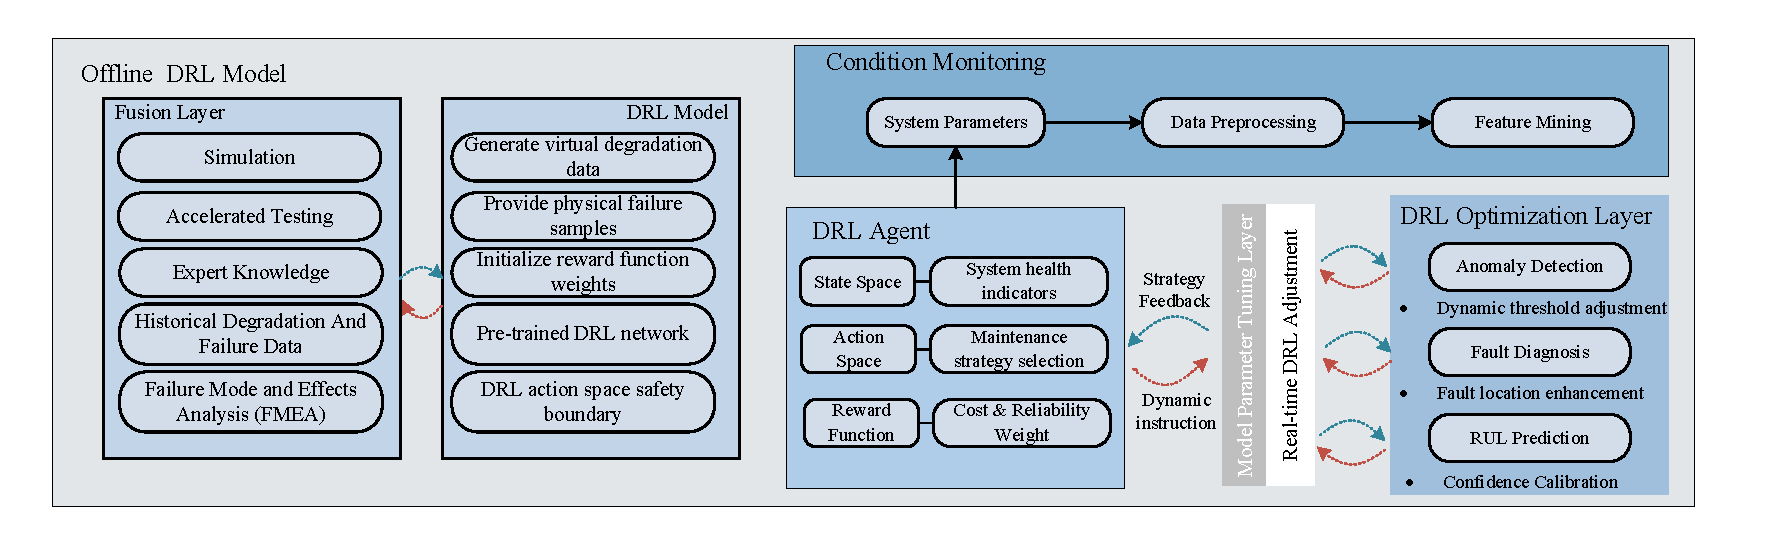
\includegraphics[width=\textwidth]{fig/maintenance.pdf}
  \caption{Workflow of DRL-based maintenance for PECs.}
  \label{fig:maintenance}
\end{figure*}


The application of DRL in converter maintenance can be categorized into three interrelated domains:
\begin{enumerate}
  \item \textbf{Condition Monitoring}: continuous tracking of converter health through sensor data and latent state representations;
  \item \textbf{Anomaly Detection and Fault Diagnosis}: identification of deviations from normal operation and localization of fault sources;
  \item \textbf{RUL Prediction}: estimation of degradation trajectories to support predictive and prescriptive maintenance decisions.
\end{enumerate}
These three domains collectively form a hierarchical pipeline that connects system observation, fault interpretation, and lifetime prediction.


In the following subsections, we review recent advances in DRL-driven techniques for each of these tasks, highlighting their methodological developments, representative applications, and implementation challenges within converter-based energy systems.

\subsection{Condition Monitoring}
\label{Condition_Monitoring}

Condition monitoring provides the foundation for intelligent maintenance in PECs by enabling continuous evaluation of system health under dynamic operating conditions. 
Traditional thresholding or statistical approaches often fail to generalize in nonlinear and time-varying environments. 
Recent research has integrated deep reinforcement learning (DRL) with deep representation learning to enhance adaptability and scalability in condition monitoring systems~\cite{xu2024comparative}. 
In particular, in multi-source energy scenarios such as residential DC microgrids and hybrid renewable systems, DRL-based agents have demonstrated the capability to extract high-level features directly from raw sensor streams and to adapt monitoring policies across varying operational regimes.

To improve generalization under limited data conditions, transfer learning and domain adaptation have been incorporated into DRL frameworks. 
Techniques such as fine-tuning and domain-adversarial neural networks (DANN) have shown significant improvement in cross-system fault recognition~\cite{saleem2024transrul}. 
For example, in HVAC systems characterized by high operational variability, DANN-based models achieved over 93\% average fault detection accuracy across multiple transfer tasks, outperforming convolutional baselines with minimal labeled data. 
Although these results were obtained in related domains, they illustrate the transferability of DRL-based condition monitoring to converter maintenance, with potential robustness against distributional shifts and hardware heterogeneity.

Furthermore, transformer architectures have recently emerged as effective models for extracting temporal dependencies and long-range correlations within operational data. 
Their self-attention mechanisms enable DRL-enhanced condition monitoring to focus adaptively on critical time intervals, improving sensitivity to early-stage degradation without requiring manually engineered features. 

By integrating DRL with transfer learning and attention-based temporal modeling, condition monitoring in PECs can achieve accurate, adaptive, and generalizable performance across diverse converter architectures and operating conditions. 
This capability establishes the foundation for subsequent tasks such as anomaly detection, fault diagnosis, and predictive maintenance.


\subsection{Anomaly Detection and Fault Diagnosis}
\label{sec:fault_diagnosis}

Building on condition monitoring, anomaly detection and fault diagnosis represent the next layer in the intelligent maintenance hierarchy of PECs. 
While condition monitoring provides passive state awareness, fault diagnosis focuses on the proactive identification of abnormal behavior, localization of failure sources, and mitigation of performance degradation. 
Conventional rule-based or model-dependent diagnostic approaches often exhibit limited robustness under nonlinear and stochastic conditions, particularly in large-scale converter networks.

DRL offers distinct advantages by learning diagnostic policies directly from complex and high-dimensional sensor data without relying on explicit physical models. 
Recent studies have integrated DRL with convolutional, recurrent, and attention-based architectures to enhance detection accuracy and real-time responsiveness. 
The integration of anomaly detection with policy optimization enables systems to not only identify faults but also determine corrective actions autonomously, paving the way toward self-healing converter infrastructures.

A representative example is a hybrid CNN–RNN DRL framework that employs convolutional layers for spatial feature extraction and recurrent units for temporal sequence modeling~\cite{nevisi2025evolutionary}. 
To further enhance adaptability, an evolutionary artificial bee colony algorithm is incorporated for hyperparameter optimization. 
Evaluations on multiple benchmark datasets, including smart grid and Pecan Street data, achieved more than 96\% classification accuracy with low variance, outperforming conventional deep learning models such as GANs, BERT, and transformers. 
The framework maintained low false alarm rates and achieved rapid convergence, demonstrating potential for real-time industrial deployment.

In multi-unit systems with economic interdependencies, DRL-based maintenance can be formulated as a condition-based optimization problem under uncertainty. 
A modified DRL algorithm for semi-Markov decision processes integrates a proportional hazards model to represent condition-dependent degradation~\cite{najafi2023deep}. 
The learned policy derives opportunistic maintenance strategies that minimize long-term costs while accounting for component aging correlations, outperforming heuristic condition-based maintenance methods in hydroelectric systems.

At the system level, predictive maintenance must coordinate both human and equipment resources. 
A DRL-based approach using PPO with long short-term memory (PPO–LSTM) networks has been developed for dynamic resource allocation in maintenance planning~\cite{ong2021deep}. 
This framework jointly detects anomalies and allocates maintenance resources, achieving 53\%–65\% improvement in maintenance efficiency compared with conventional strategies in simulation environments.

In specialized domains such as electromagnetic susceptibility testing, DRL has been applied to design excitation waveforms that expose converter vulnerabilities~\cite{chen2024determining}. 
Using a TD3 algorithm with reward shaping, the agent autonomously adjusts waveform parameters to trigger fault responses, achieving faster convergence and higher detection sensitivity than heuristic or standard waveforms. 
Reinforcement learning has also been employed for active excitation design in system identification. 
An RL-based framework proposed in~\cite{huang2023reinforcement} generates excitation signals that maximize parameter identifiability for Li-ion battery systems—a methodology extendable to converter components such as inductors and capacitors.

Collectively, these developments demonstrate that DRL-based fault diagnosis unifies perception, decision-making, and maintenance scheduling within a single data-driven framework. 
Nevertheless, challenges remain regarding policy interpretability, limited fault data availability, and the realization of real-time performance under embedded hardware constraints.


\subsection{RUL Prediction}
\label{sec:rul_prediction}

Building upon anomaly detection and fault diagnosis, the final stage in a data-driven maintenance pipeline involves predicting the RUL of critical components. 
Accurate RUL estimation is essential for predictive maintenance, which aims to optimize component utilization, prevent catastrophic failures, and minimize unplanned downtime in converter-based systems. 
Traditional model-based methods often require extensive parameterization and exhibit limited adaptability to varying stress conditions, whereas recent advances in DRL and transformer-based architectures provide data-driven alternatives capable of capturing degradation patterns directly from operational data.

A representative study applies DRL to the degradation-aware control of solid-state transformers, which are key components in high-power converter systems. 
In~\cite{haque2021deep}, an actor–critic DDPG controller dynamically adjusts the phase-shift angle according to real-time health indicators, eliminating the need for explicit degradation models. 
Experimental validation on a 5~kW GaN-based SST prototype demonstrated that the controller effectively balances power delivery and device stress, establishing a practical pathway for RUL-integrated control strategies in mission-critical converter applications.

In parallel, sequence modeling techniques based on transformers have achieved significant progress in RUL prediction for battery-powered converter systems. 
In~\cite{saleem2024transrul}, a dual-encoder transformer model estimates the RUL of lithium-ion batteries using multi-head attention and positional encoding to capture long-term dependencies and nonlinear aging behaviors. 
The proposed Trans-RUL framework outperformed convolutional baselines on the CALCE CS\textsubscript{2} dataset in terms of mean absolute error, root mean square error, and coefficient of determination, while maintaining a lightweight structure suitable for embedded, real-time applications.

Together, these studies highlight two complementary directions for RUL prediction in PECs:
\begin{enumerate}
  \item \textbf{Control-integrated degradation modeling}, where DRL dynamically adjusts operating parameters to extend component lifetime while maintaining system performance;
  \item \textbf{Sequence-based lifetime estimation}, where transformer architectures capture temporal degradation trajectories for accurate lifetime prediction.
\end{enumerate}

These approaches collectively advance converter maintenance toward intelligent, resilient, and autonomous lifecycle management.


\subsection{Discussion}
\label{sec:maintenance_discussion}

DRL-enabled maintenance strategies represent a transformative advancement in the reliability engineering of PECs.
Across the three major domains, including condition monitoring, anomaly detection and fault diagnosis, and RUL prediction, DRL provides a unified framework for continuous learning, adaptive decision-making, and real-time operation.
Condition monitoring benefits from attention-based temporal modeling and domain transfer learning, enabling accurate and generalizable system state perception. 
Anomaly detection and fault diagnosis leverage the capability of DRL for policy optimization and sequential reasoning, enabling early and autonomous fault identification even under heterogeneous and imbalanced data conditions.
RUL prediction integrates reinforcement learning and deep sequence modeling to estimate component lifetime and support proactive maintenance scheduling.

Collectively, these developments mark a paradigm shift from reactive or scheduled maintenance to intelligent, data-driven predictive maintenance, improving operational efficiency, reliability, and lifecycle cost. 
However, several challenges remain, including limited sample efficiency, policy interpretability, data imbalance, and real-time execution on embedded hardware. 
Future research may focus on hybrid DRL–physics-informed models, federated learning for cross-device generalization, and runtime assurance frameworks to ensure safety and certification. 
These directions are expected to accelerate the transition from laboratory prototypes to large-scale industrial deployment of DRL-enabled maintenance in converter-based energy systems.

